% \setchapterpreamble[u]{\margintoc}
\chapter{Process Management}
\labch{procman}

\section{What is sleep?}

\lstinline|sleep| is a command that is used to delay the execution of a process
for a specified amount of time. \textbf{sleep} itself is a no-op command,
\footnote{
  NO-OP stands for No Operation. It is a command that does nothing.
  More reading on NO-OP can be found
  \href{https://en.wikipedia.org/wiki/NOP\_(code)}{here}.
}
but it takes a variable amount of time to execute, depending on the argument
of the command. This is useful when you want to delay the execution of another
command or chain of commands by a certain amount of time.

\subsection{Example}

\begin{lstlisting}[language=bash]
$ sleep 5
$ echo "Hello, World!"
Hello, World!
\end{lstlisting}

\subsection{Scripting with sleep}

If you run the above snippet, you will see that the output is delayed by 5 seconds.
Moreover, the prompt itself will not be available for 5 seconds, as the shell is busy
with executing the \lstinline|sleep| command.
To run the entire snippet as one process, simply put the two commands on
separate lines of a file (say, \lstinline|hello.sh|), and run the file as a script.

\begin{lstlisting}[language=bash]
$ cat hello.sh
sleep 5
echo "Hello, World!"
$ bash hello.sh
Hello, World!
\end{lstlisting}

We will be using \lstinline|sleep| in the examples throughout this chapter to demonstrate
process management since it is a simple command that can be used to quickly
spawn an idempotent process for any arbitrary amount of time.

\subsection{Syntax and Synopsis}

\begin{lstlisting}[language=bash]
sleep NUMBER[SUFFIX]...
\end{lstlisting}

Here the \lstinline|NUMBER| is the amount of time to sleep.
The \lstinline|SUFFIX| can be \lstinline|s| for seconds, \lstinline|m| for minutes,
\lstinline|h| for hours, and \lstinline|d| for days.

\vfill
\pagebreak
\section{Different ways of running a process}

\subsection{What are processes?}

\begin{definition}[Process]
  A process is an instance of a program that is being executed.
  It contains the program code and its current activity.
  Depending on the operating system (OS), a process may be made up of
  multiple threads of execution that execute instructions concurrently.
  Several processes may be associated with the same program; for example,
  opening up several instances of the same program often means more than
  one process is being executed.
  Each process has its own `process id` or \textbf{PID} to uniquely identify it.
\end{definition}

Whenever we run an application, or even a command on the linux shell, it spawns a process. Processes are always created by an already
existing process
\sidenote{
  Other than the very first process, which is always the
  \textbf{init} process. In most distributions, this is
  done by
  \href{https://systemd.io/}{systemd}, which is an
  init system that does a lot of other things as well.
  You can learn more about systemd and what all
  it does
  \href{https://documentation.suse.com/external-tree/en-us/sles/12-SP4/systemd\_in\_suse\_linux\_enterprise\_12\_white\_paper.pdf}{here}.
}
This creates a tree-like structure of processes, where each process has a parent process and can have multiple child processes.
When the parent of a process dies, the child processes are adopted by the \textbf{init} process.
\textbf{init} is thus the root of the process tree.

\begin{figure}[h!]
  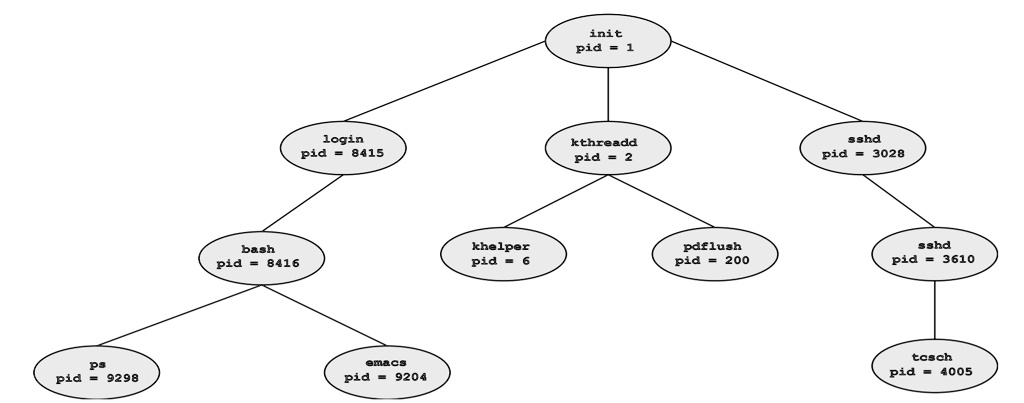
\includegraphics{process-tree}
  \caption{Example of a process tree}
  \labfig{process-tree}
\end{figure}

\subsection{Process Creation}
In linux systems, processes are managed by the kernel.
The kernel is responsible for creating, scheduling, and destroying processes.
The user can interact with the kernel using system calls to create, manage, and destroy processes.
Creating processes is simple, and can be done using the \textbf{fork()} system call.
This is used when any process wants to create a new process.

To simply create a new process for a command,
we can simply type in the command and press enter.
This will not only fork a new process from the terminal or
terminal emulator as the parent process, but also tie the
standard input, standard output, and standard error of the child process
to the terminal or terminal emulator.
\sidenote{
  Standard Input, Output, and Error are the default streams that are used by
  the shell to interact with the user. Standard Input is used to take input from
  the user, Standard Output is used to display output to the user, and Standard Error
  is used to display errors to the user. We will cover these in details in the next chapter.
}

\begin{lstlisting}[language=bash]
$ sleep 5
\end{lstlisting}

This will create a new process that will sleep for 5 seconds.

Remember that each process has a unique process id (PID).
Each process also has a parent process id (PPID),
which is the PID of the parent process.
If a process is created by the shell, the shell will be the parent process.
If the shell's process is killed, the child process will also
be killed, as the child process is owned by the shell.

\subsection{Process Ownership}

If you are using a linux operating system with a GUI server (X or Wayland),
try the following to understand how process ownership works.

Open two terminals, in the first one, run \lstinline|echo \$\$| to see the
process ID of that shell.
It should print out a random string of digits, that is the PID of the shell.
Then run a GUI application, such as \textbf{firefox}.
\sidenote{
  Make sure you are running something that is not running already.
}
This will block your terminal and open a new window of firefox.

\begin{lstlisting}[language=bash]
$ echo $$
2277503
$ firefox
\end{lstlisting}

Now in the other terminal, which is free, run \lstinline|pgrep firefox|
\sidenote{
  or whatever was your process's name
}
It should print out another random string of digits, it is the PID of
firefox.

Now you can use the following command to find the parent process's process
ID (PPID) to verify it is the same as the output of \lstinline|$$| in the first terminal.

\begin{lstlisting}[language=bash]
$ pgrep firefox
2278276
$ ps -efj | awk '$2==2278276;NR==1'
UID          PID    PPID    PGID     SID  C STIME TTY          TIME CMD
sayan    2278276 2277503 2278276 2277503 12 16:59 pts/5    00:00:03 /usr/lib/firefox/firefox
\end{lstlisting}

Here we can see that the PPID of firefox is the PID of the shell.

Note that the second command should put the PID of firefox, which we got
from the previous command. This can also be done in a single command
which you can directly copy and paste in your terminal.

\begin{lstlisting}[language=bash]
$ ps -efj | awk "\$2==$(pgrep firefox);NR==1"
UID          PID    PPID    PGID     SID  C STIME TTY          TIME CMD
sayan    2278276 2277503 2278276 2277503  1 16:59 pts/5    00:00:04 /usr/lib/firefox/firefox
\end{lstlisting}

Now, what happens if we kill the parent process?
To kill a process all we need to use is use the \lstinline|kill|
command with the PID of the process.

\begin{lstlisting}[language=bash]
$ kill -9 2277503
\end{lstlisting}

\marginnote{
  The \lstinline|-9| flag is used to send a \textbf{SIGKILL} signal to the process.
  This signal is used to kill a process immediately.
  We will cover signals later.
}

If you have been following along, you will see that both the terminal and firefox
dissapear from your screen. You will also notice that if you run the same
command to print the PID and PPID of firefox, it does not show anything.
This is because the process is killed and the process tree is destroyed, so
even firefox, being the child of the shell process, is killed.

\subsection{Don't kill my children}

However, there are also ways to create a new process in the background.
The easiest way to do this is to append an ampersand (\lstinline|&|) to the
end of the command. This is a shell syntax that tells the shell to fork the
command as a child process and run it in the background. What this means is
the shell will not wait for the command to finish, and will return the prompt
to the user immediately. However, the standard output and standard error may
still be tied to the terminal or terminal emulator. So if the process writes
something to the standard output or standard error, it will be displayed on the
terminal. Furthermore, the process is still owned by the shell, and if the shell
is killed, the process's parent will be changed to the \textbf{init} process.

Lets try the same exercise as earlier, but now with the \lstinline|&| at the end.

Open two terminals, and in the first one, execute the following command.

\begin{lstlisting}[language=bash]
$ echo $$
2400520
$ firefox &
[1] 2401297
$ echo "hello"
hello
$
ATTENTION: default value of option mesa_glthread overridden by environment.
$
\end{lstlisting}

You can observe that the firefox window opens up similar to last time, but
now the prompt returns immediately. You can also see that the output of the
\lstinline|echo| command is displayed on the terminal.

If you try to perform some operations in the browser, it may also print
some messages to the terminal screen, even though it is not waiting for
the command to finish. The "ATTENTION" message is an example of this.

Also observe that as soon as we launched \textbf{firefox}, it printed out
two numbers, [1] and 2401297. The number in the square brackets is the job
id of the process, and the number after that is the PID of the process.
So now we dont even need to use \lstinline|pgrep| to find the PID of the process.

Now in the other terminal, run the following command.

\begin{lstlisting}[language=bash]
$ ps -efj | awk "\$2==$(pgrep firefox);NR==1"
UID          PID    PPID    PGID     SID  C STIME TTY          TIME CMD
sayan    2401297 2400520 2401297 2400520  3 17:13 pts/5    00:00:08 /usr/lib/firefox/firefox
\end{lstlisting}

Still we can see that the PPID of firefox is the PID of the shell.

Now, if we kill the parent process, the child process will be adopted by the
init process, and will continue to run.

\begin{lstlisting}[language=bash]
$ kill -9 2400520
\end{lstlisting}

If you re-run the command to print the PID and PPID of firefox, you will see
that the PPID of firefox is now set to $1$, which is the PID of the \textbf{init}
command.

\begin{lstlisting}[language=bash]
$ ps -efj | awk "\$2==$(pgrep firefox);NR==1"
UID          PID    PPID    PGID     SID  C STIME TTY          TIME CMD
sayan    2401297       1 2401297 2400520  3 17:13 ?        00:00:09 /usr/lib/firefox/firefox
\end{lstlisting}

You can also see that the TTY column is now set to \lstinline|?|, which means that
the process is no longer tied to the terminal.

However, if instead of killing the parent process using the \textbf{SIGKILL}
signal, if you sent the \textbf{SIGHUP} signal to the parent, the child process
will still be terminated, as it will propagate the hangup signal to the child process.


\subsection{Setsid}

So how do we start a process directly in a way that it is not tied to the terminal?
Many times we would require to start a process in the background to run
asynchronously, but not always do we want to see the output of the process
in the terminal from where we launched it. We may also want the process
to be owned by the \textbf{init} process from the get go.

To do this, we can use the \lstinline|setsid| command. This command is used to
run a command in a new session. This will create a new process group and
set the PPID of the process to the \textbf{init} process. The TTY will also
be set to \lstinline|?|.

Lets try the same exercise with the \lstinline|setsid| command.
Open two terminals, in one of them, run the following command.

\begin{lstlisting}[language=bash]
$ echo $$
2453741
$ setsid -f firefox
$
\end{lstlisting}

Observe that firefox will open up, but the prompt will return immediately.

In another terminal, run the following command.

\begin{lstlisting}[language=bash]
$ ps -efj | awk "\$2==$(pgrep firefox);NR==1"
UID          PID    PPID    PGID     SID  C STIME TTY          TIME CMD
sayan    2454452       1 2454452 2454452  2 17:19 ?        00:00:07 /usr/lib/firefox/firefox
\end{lstlisting}

Observe that even without killing the parent process, the PPID of firefox is
already set to $1$, which is the PID of the \textbf{init} process.
So the process will not be killed if the shell is killed.

This is called a hang-up signal. We can still artificially send the
\textbf{SIGHUP} signal, which tells firefox that its parent has stopped
by using the \lstinline|kill -1| command.

\begin{lstlisting}[language=bash]
$ kill -1 2454452
\end{lstlisting}

This will still close firefox, even though the parent process (\textbf{init})
didn't actually get killed.

\subsection{Nohup}

If you do not want to give up the ownership of a child process,
and also don't really need to get the prompt back, but you do not
want to see the output of the command in your terminal. You can
use the \lstinline|nohup| command followed by the command you want to
run. It will still be tied to the terminal, and you can use
\lstinline|Ctrl+C| to stop it, \lstinline|Ctrl+Z| to pause it, etc.
The prompt will also be blocked till the process runs.
However, the input given to the terminal will not be sent
to the process, and the output of the process will not be
shown on the terminal. Instead, the output will be saved
in a file named \lstinline|nohup.out| in the current directory.

However, this is different from simply running the command
with a redirection operator (\lstinline|>|) at the end,
\sidenote{
  We will cover redirection operators in the next chapter.
}
because the \lstinline|nohup| command also makes the process
immune to the hang-up signal.

\begin{exercise}
  Try the same exercise as before, but this time use the \lstinline|nohup|
  to run firefox, then in another terminal, find the PID and PPID of
  firefox. Then try to kill the parent process and see if firefox
  dies or not.
\end{exercise}

\subsection{coproc}

The \lstinline|coproc| command is used to run a command in the background
and tie the standard input and standard output of the command to a
file descriptor. This is useful when you want to run a command in the
background, but still want to interact with it using the shell.
This creates a two way pipe between the shell and the command.

\textbf{Syntax}

\begin{lstlisting}[language=bash]
$ coproc [NAME] command [redirections]
\end{lstlisting}

This creates a coprocess named \lstinline|NAME| and runs the command in the background.
If the \lstinline|NAME| is not provided, the default name is \lstinline|COPROC|.

However, the recommended way to use \lstinline|coproc| is to use it in a
subshell, so that the file descriptors are automatically closed when
the subshell exits.

\begin{lstlisting}[language=bash]
$ coproc [NAME] { command; }
\end{lstlisting}

coproc can execute simple commands or compound commands. For simple
commands, name is not possible to be specified. Compound commands like
loops or conditionals can be executed using coproc in a subshell.

The name that is set becomes a array variable in the shell, and can be used
to access the file descriptors for stdin, stdout, and stderr.

For example, to provide input to the command, you can use \lstinline|echo| and
redirection operators to write to the file descriptor.

Similarly you can use the \lstinline|read| command to read from the file descriptor.

\begin{lstlisting}[language=bash]
$ coproc BC { bc -l; }
$ jobs
[1]+  Running                 coproc BC { bc -l; } &
$ echo 22/7 >&"${BC[1]}"
$ read output <&"${BC[0]}"
$ echo $output
3.14285714285714285714
\end{lstlisting}

This uses concepts from redirection and shell variables, which we will cover
in later weeks.

\subsection{at and cron}

Processes can also be scheduled to be launched at a later time.
This is usually done using \textbf{cron} or the \textbf{at} command.
We will cover these in depth later.

\subsection{GNU parallel}

GNU parallel is a shell tool for executing jobs in parallel using one
or more computers. A job can be a single command or a small script that
has to be run for each of the lines in the input. The typical input is
a list of files, a list of hosts, a list of users, a list of URLs, or a
list of tables. A job can also be a command that reads from a pipe.
GNU parallel can then split the input into blocks and pipe a block
into each command in parallel.

\subsection{systemd services}

Finally, the best way to run a background process or a daemon is to use
\textbf{systemd} services. \textbf{systemd} is an init system that is
used by most modern linux distributions. You can create a service file
declaring the process, the command line arguments, the environment variables,
and the user and group that the process should run as. You can also
specify if the process should be restarted if it crashes, or if it should
be started at boot time.


\vfill
\pagebreak
\section{Process Management}
\subsection{Disown}

Disown is a shell builtin command that is used to remove a job from the shell's
job table. This is useful when you have started a process in the background
and you want to remove it from the shell's job table, so that it is not
killed when the shell is killed. What it means is that if the parent
process recieves a hang-up signal, it will not propagate it to the child
job if it is removed from the job table.
This is applicable only for processes started from a shell.

Open two terminals, in one, open firefox in background using the \lstinline|&|

\begin{lstlisting}[language=bash]
$ firefox &
$
\end{lstlisting}

and then in the other terminal, run the following command.

\begin{lstlisting}[language=bash]
$ ps -efj | awk "\$2==$(pgrep firefox);NR==1"
UID          PID    PPID    PGID     SID  C STIME TTY          TIME CMD
sayan    3216429 3215856 3216429 3215856 69 18:45 pts/5    00:00:02 /usr/lib/firefox/firefox
$ kill -1 3215856
\end{lstlisting}

Observe that firefox will close, even though it was running in the background.
This is because the shell will propagate the hang-up signal to the child process.
If the parent shell was forcefully killed using the \textbf{SIGKILL} signal,
then it wont have the opportunity to propagate the hang-up signal to the child process.
This is a separate process than the natural killing of firefox running in
foreground even when shell is killed with \textbf{SIGKILL} signal.

Now, to fix this, we can simply run the \lstinline|disown| command in the terminal
where we started the firefox process.

Again open a terminal emulator and run the following command.

\begin{lstlisting}[language=bash]
$ firefox &
$ disown
$
\end{lstlisting}

Now, in the other terminal, run the following command.

\begin{lstlisting}[language=bash]
$ ps -efj | awk "\$2==$(pgrep firefox);NR==1"
UID          PID    PPID    PGID     SID  C STIME TTY          TIME CMD
sayan    3216429 3215856 3216429 3215856 69 18:45 pts/5    00:00:02 /usr/lib/firefox/firefox
$ kill -1 3215856
$ ps -efj | awk "\$2==$(pgrep firefox);NR==1"
UID          PID    PPID    PGID     SID  C STIME TTY          TIME CMD
sayan    3216429       1 3216429 3215856 10 18:45 ?        00:00:03 /usr/lib/firefox/firefox
\end{lstlisting}

Firefox does not close anymore, even when the parent process is hanged up.

\subsection{Jobs}

To list the jobs that are running in a shell, you can use the \lstinline|jobs| command.

\begin{lstlisting}[language=bash]
$ firefox &
$ sleep 50 &
$ jobs
[1]-  Running                 firefox &
[2]+  Running                 sleep 50 &
\end{lstlisting}

Here \lstinline|+| denotes the current job, and \lstinline|-| denotes the previous job.
The first column is the job number, it can also be used to refer to the job
inside that same shell. The process ID of a process can be used to refer to
the process from anywhere, but the job ID is only valid in the shell where
it is created.

The process id can be listed using the \lstinline|jobs -l| command.

\begin{lstlisting}[language=bash]
$ jobs -l
[1]- 3303198 Running                 firefox &
[2]+ 3304382 Running                 sleep 50 &
\end{lstlisting}

Using disown removes the job from this table. We can selectively
remove only some jobs from the table as well.

\begin{lstlisting}[language=bash]
$ jobs
[1]-  Running                 firefox &
[2]+  Running                 sleep 50 &
disown %1
$ jobs
[2]+  Running                 sleep 50 &
\end{lstlisting}

Whereas using \lstinline|disown -a| will remove all jobs from the table.
\lstinline|disown -r| will remove only running jobs from the table.

If you dont really want to lose the job from the table, but you want to
prevent it from being killed when the shell is killed, you can use
\lstinline|disown -h| to mark the jobs to be ignored by the hang-up signal.
It will have same effect as last exercise, but it will still be present
in the output of the \lstinline|jobs| command.

\subsection{Suspending and Resuming Jobs}

Sometimes you may want to pause a job and resume it later.
This is supported directly by the linux kernel.
To pause any process you can send it the \textbf{SIGSTOP} or \textbf{SIGTSTP} signal.
\sidenote{
  The difference between \textbf{SIGSTOP} and \textbf{SIGTSTP} is that
  \textbf{SIGSTOP} is a signal that cannot be caught or ignored by the process,
  so the process will be paused immediately. \textbf{SIGTSTP} is a signal that
  can be caught or ignored by the process, so the process can do some cleanup
  before pausing. The default action of \textbf{SIGTSTP} is to pause the process.
}
This can be done using the same \textbf{kill} command. The signal number for
\textbf{SIGSTOP} is 19, and for \textbf{SIGTSTP} is 20.

To resume the process, you can send it the \textbf{SIGCONT} signal.
The signal number for \textbf{SIGCONT} is 18.

\begin{exercise}
  Try to pause a job using the \textbf{SIGSTOP} signal, then resume it using the
  \textbf{SIGCONT} signal.
  Open firefox from a terminal using \lstinline|firefox \&| and note the PID,
  then pause it using
  \lstinline|kill -19 <PID>|,
  try to click on the firefox window, and see if it responds.
  Then resume it using \lstinline|kill -18 <PID>|.
  Does the firefox window respond now?
\end{exercise}

If you start a command from the shell without using the \lstinline|&| operator,
you can pause the command using \lstinline|Ctrl+Z| and resume it using the
\lstinline|fg| command.
This sends the same signals as above, and uses the shell's job table
to keep track of the jobs.

\begin{remark}
  Just like disown, the \lstinline|fg| command can also take the job number
  as an argument to bring that job to the foreground. The default job
  is the current job. (Marked with a \lstinline|+| in the \lstinline|jobs| command))
\end{remark}

You can also use the \lstinline|bg| command to resume a job, but in the background.
This has same effect as using the \lstinline|&| operator at the end of the command.

\begin{remark}
  Since the disown, fg, and bg commands work on the shell's job table,
  they are shell builtins, and not a executable binary.
  You can verify this using the \lstinline|type| command.
\end{remark}

You cannot perform job control on a process that is not started from the shell,
or if you have disowned the process.

\subsection{Killing Processes}

We have been using the \lstinline|kill| command to send signals to processes.
The kill command is a shell builtin and an executable command that is used
to send signals to processes. The default signal that is sent is the
\textbf{SIGTERM} signal, which is signal number 15.
The kill command is the user-land way to communicate with the kernel that
some process needs to be given a certain signal.

\textbf{Syntax}

\begin{lstlisting}[language=bash]
$ kill [-signal|-s signal] PID|name...
\end{lstlisting}

Let us also briefly discuss what the synopsis of the command means, and
how to interpret it.

The first word is the name of the command, which is \lstinline|kill| in this case.
The argument \textbf{signal} inside square brackets means that it is optional.
The argument \textbf{PID} is the process ID of the process that you want to kill.
The argument \textbf{name} is the name of the process that you want to kill.
The pipe between \textbf{PID} and \textbf{name} means that you can provide
either the PID or the name of the process.
The ellipsis (\lstinline|...|) after \textbf{PID|name} means that you can provide
as many PIDs or names as you want.

\begin{remark}
  As mentioned, kill is also a shell builtin command. This means that
  the synopsis seen in the man page of kill is not the same as the
  synopsis of the builtin. The bash builtin of kill does not support
  providing names of the processes, only the PIDs. Hence if you want
  to kill a process by its name, you will either have to use the
  path of the kill binary, or use the \lstinline|pkill| command.
\end{remark}

So for example, we can run kill in the following manners.

\begin{lstlisting}[language=bash]
$ kill 2452
$ kill -9 2452
$ kill -9 2452 62
$ kill -SIGKILL 2525
$ kill -SIGKILL 2525 732
\end{lstlisting}

The \lstinline|kill| command can also be used to send other non-terminating signals
to the process. For example, the \textbf{SIGSTP} signal can be used to pause
a process, and the \textbf{SIGCONT} signal can be used to resume a process.
Similarly, there are some undefined signals that can be used to send custom
signals to the process.

\textbf{SIGUSR1} and \textbf{SIGUSR2} are signals that do not have any predefined
behaviour, and can be used by the user to send custom signals to the process.
The behaviour of the process on receipt of these signals is decided by the
process and told to the user by the process documentation. The user can
then send these signals to the process using the \lstinline|kill| command.
This helps user interact with processes that are not running directly in the
foreground of a shell.

Processes can also \textbf{trap} signals, which means that they can catch
a signal and run a custom handler function. This is useful when you want
to do some cleanup before the process is killed. This can also be used
to totally change how the process behaves on receipt of a signal.
However, to prevent malicious code from running, the \textbf{SIGKILL} signal
cannot be trapped, and the process will be killed immediately. Similarly
the \textbf{SIGSTOP} signal, which is similar in definition to the \textbf{SIGSTP}
signal, cannot be trapped.

To see the list of the signals, we can run \lstinline|kill -l|.

\begin{lstlisting}[language=bash]
$ kill -l
 1) SIGHUP       2) SIGINT       3) SIGQUIT      4) SIGILL       5) SIGTRAP
 6) SIGABRT      7) SIGBUS       8) SIGFPE       9) SIGKILL     10) SIGUSR1
11) SIGSEGV     12) SIGUSR2     13) SIGPIPE     14) SIGALRM     15) SIGTERM
16) SIGSTKFLT   17) SIGCHLD     18) SIGCONT     19) SIGSTOP     20) SIGTSTP
21) SIGTTIN     22) SIGTTOU     23) SIGURG      24) SIGXCPU     25) SIGXFSZ
26) SIGVTALRM   27) SIGPROF     28) SIGWINCH    29) SIGIO       30) SIGPWR
31) SIGSYS      34) SIGRTMIN    35) SIGRTMIN+1  36) SIGRTMIN+2  37) SIGRTMIN+3
38) SIGRTMIN+4  39) SIGRTMIN+5  40) SIGRTMIN+6  41) SIGRTMIN+7  42) SIGRTMIN+8
43) SIGRTMIN+9  44) SIGRTMIN+10 45) SIGRTMIN+11 46) SIGRTMIN+12 47) SIGRTMIN+13
48) SIGRTMIN+14 49) SIGRTMIN+15 50) SIGRTMAX-14 51) SIGRTMAX-13 52) SIGRTMAX-12
53) SIGRTMAX-11 54) SIGRTMAX-10 55) SIGRTMAX-9  56) SIGRTMAX-8  57) SIGRTMAX-7
58) SIGRTMAX-6  59) SIGRTMAX-5  60) SIGRTMAX-4  61) SIGRTMAX-3  62) SIGRTMAX-2
\end{lstlisting}

Some of the important signals are:

\begin{itemize}
  \item \textbf{SIGHUP} - Hangup signal. This is sent to a process when the
  terminal is closed. This is used to tell the process that the terminal
  is no longer available.
\item \textbf{SIGINT} - Interrupt signal. This is sent to a process when the
  user presses \lstinline|Ctrl+C|. This is used to tell the process to stop
  what it is doing and exit.
\item \textbf{SIGKILL} - Kill signal. This is used to kill a process immediately.
  This signal cannot be caught or ignored by the process.
\item \textbf{SIGTERM} - Terminate signal. This is used to tell the process
  to exit gracefully. The process can catch this signal and do some cleanup
  before exiting. This is the default signal sent by the \lstinline|kill| command.
\item \textbf{SIGSTP} - Stop signal. This is used to pause a process.
  This is sent when the user presses \lstinline|Ctrl+Z|. This signal can be
  caught or ignored by the process.
\item \textbf{SIGSTOP} - Stop signal. This is used to pause a process.
  This signal cannot be caught or ignored by the process.
\item \textbf{SIGCONT} - Continue signal. This is used to resume a process
  that has been paused using the \textbf{SIGSTOP} signal. This is sent
  when the user presses \lstinline|fg| or \lstinline|bg|.
\item \textbf{SIGUSR1} - User defined signal 1. This is a signal that can
  be used by the user to send a custom signal to the process.
\item \textbf{SIGUSR2} - User defined signal 2. This is a signal that can
  be used by the user to send a custom signal to the process.
\item \textbf{SIGCHLD} - Child signal. This is sent to the parent process
  when a child process exits. This is used to tell the parent process that
  the child process has exited.
\item \textbf{SIGSEGV} - Segmentation fault signal. This is sent to a process
  when it tries to access memory that it is not allowed to access.
\item \textbf{SIGPIPE} - Pipe signal. This is sent to a process when it tries
  to write to a pipe that has been closed.
\end{itemize}

\vfill
\pagebreak
\section{Finding Processes}

As we saw, managing a process is easy once we know the PID of the process.
However, it is not always easy to find the PID of a process.
To do this, there are multiple tools in linux that can be used.

\subsection{pgrep}

The \lstinline|pgrep| command is used to find the PID of a process based on its name.
It can take the name of the process as an argument, and will print the PID of the
processes that match the name. The search can also be a regex pattern.
\sidenote{
  We will discuss regex patterns in the next chapter.
}
We have already seen how \lstinline|pgrep| can be used to find the PID of a process.

\begin{lstlisting}[language=bash]
$ pgrep firefox
526272
\end{lstlisting}

We can also use it for any process run from the terminal.

\begin{lstlisting}[language=bash]
$ sleep 50 &
$ sleep 20 &
$ sleep 10 &
$ pgrep sleep
98963
99332
99526
\end{lstlisting}

\subsection{pkill}

Similarly, we also have the \lstinline|pkill| command, which is used to kill a process
based on its name. It can take the name of the process as an argument, and will
send the \textbf{SIGTERM} signal to the processes that match the name.
Other signals can also be sent using the \lstinline|-signal| flag, similar to the
kill command.

\begin{lstlisting}[language=bash]
$ pkill firefox
\end{lstlisting}

\subsection{pidwait}

The \lstinline|pidwait| command is used to wait for a process to exit.
It searches for the process using its name, a part of its name, or any
regex matching its name, and waits for the process to exit.

\begin{exercise}
  Open firefox from a terminal in the background, then use the \lstinline|pidwait|
  to wait till the process exits. After some time, close the firefox window
  and observe the terminal.
\end{exercise}

\vfill
\pagebreak
\section{Listing Processes}

Sometimes we may not even know the name of the process, and we may want to
list all the processes running on the system. This can be done using the
many commands.

\subsection{ps}

\textbf{ps} is an ancient command
\sidenote{
  It exists in the Unix V7 manual, which was released in 1979.
  It has BSD-like options, GNU-like options, and System V-like options.
}
that is used to list the processes running on the system.

There are a lot of options and flags that can be used with the \textbf{ps} command.
The flags are of multiple types, and some flags perform the same function but
are named differently. This is because the \textbf{ps} command has been around
for a long time, and has been implemented in multiple ways in different systems.
There are also different formats in which the output can be displayed.

The most common flags used with the \textbf{ps} command are:

\begin{itemize}
  \item \textbf{ps} - This will get a snapshot of the processes owned by the user tied to the TTY.
  \item \textbf{ps -e} - This will show all the processes.
  \item \textbf{ps -f} - This will show full format listing.
  \item \textbf{ps -l} - This will show long format listing.
  \item \textbf{ps u} - This will show user-oriented format listing.
  \item \textbf{ps x} - This will show processes without controlling terminals.
  \item \textbf{ps -A} - This will show all processes.
  \item \textbf{ps aux} - This is a common command to see all processes owned by all users with and without TTY associations and showing the user who owns them.
  \item \textbf{ps --forest} - This will show the processes in a tree form.
\end{itemize}

There are hundreds of flags that can be used with the \textbf{ps} command.

\begin{exercise}
  Try to use the \textbf{ps} command with the flags mentioned above, and see
  the output of the command.
\end{exercise}

\subsection{pstree}

The \textbf{pstree} command is used to display the processes in a tree form.
Although the \textbf{ps} command can also display the processes in a tree form
using the \lstinline|--forest| flag, the \textbf{pstree} command is more suited
for this purpose. It has many features that ps lacks, such as collapsing
branches of identical processes, better ASCII art, Unicode support, etc.

If the system and the terminal supports unicode, the \textbf{pstree} command
will automatically use
\href{https://en.wikipedia.org/wiki/Box-drawing\_character}{VT100 box-drawing characters}
to make the tree look better. We can still force it to use ASCII with the
\lstinline|-A| flag.

We can also disable the clubbing of identical processes using the \lstinline|-c| flag.

The pstree command optionally takes a PID as an argument, and will display
the tree rooted at that PID. If no PID is provided, it will display the
tree rooted at the init process.

I can find the PID of the tmux server I am running to develop this book
using the \lstinline|pgrep| command.
\begin{lstlisting}[language=bash]
$ pgrep tmux
62957
\end{lstlisting}

And then use the \lstinline|pstree| command
to display the tree rooted at that PID.

\begin{lstlisting}[language=bash]
$ pstree -A 62957
tmux: server-+-bash---nvim-+-nvim-+-node---14*[{node}]
             |             |      |-texlab---9*[{texlab}]
             |             |      |-xsel
             |             |      `-9*[{nvim}]
             |             `-2*[{nvim}]
             |-bash---watch.sh---entr
             |-bash---zathura---8*[{zathura}]
             |-3*[bash]
             |-2*[bash---man---less]
             |-bash---nvim-+-nvim-+-2*[node---9*[{node}]]
             |             |      `-{nvim}
             |             `-2*[{nvim}]
             `-bash-+-pstree
                    `-xsel
\end{lstlisting}

This helps us easily find out which processes are running under which process,
and helps us understand the process tree.

\subsection{top}

The \textbf{top} command is used to display the processes that are running
in real time. It is an interactive command that displays the processes in
a table format, and updates the table every few seconds. It also displays
the CPU and memory usage of the processes.

The \textbf{top} command is very useful when you want to monitor the processes
and the resources they are using in real time. It is also useful when you
want to find out which process is using the most CPU or memory.

Since it is an interactive command, it has keyboard shortcuts as well, along
with runtime options that can be used to change the behaviour of the command.

\marginnote{
  Note: The output of the \textbf{top} command is not static, and it contains
  control characters and
  \href{https://en.wikipedia.org/wiki/ANSI\_escape\_code}{ANSI escape codes}
  to make the output beautiful and interactive. This is why the output is not
  suitable for use in scripts, and is only meant for human consumption.
  I have removed the control characters and ANSI escape codes from the output
  shown here.
}

\begin{lstlisting}
$ top
top - 15:44:55 up 40 min,  1 user,  load average: 2.03, 1.37, 1.02
Tasks: 271 total,   1 running, 270 sleeping,   0 stopped,   0 zombie
%Cpu(s):  9.8 us,  4.9 sy,  0.0 ni, 85.4 id,  0.0 wa,  0.0 hi,  0.0 si,  0.0 st
MiB Mem :   7764.2 total,    604.5 free,   5663.2 used,   1919.6 buff/cache
MiB Swap:  20002.0 total,  19901.2 free,    100.8 used.   2101.0 avail Mem

    PID USER      PR  NI    VIRT    RES    SHR S  %CPU  %MEM     TIME+ COMMAND
    631 sayan     20   0 1248084  81976  44580 S  18.2   1.0   1:39.82 Xorg
   1072 sayan     20   0 3159356 229336  89816 S   9.1   2.9   0:44.01 spotify
   1079 sayan     20   0 1123.5g 128252  65776 S   9.1   1.6   0:09.37 Discord
      1 root      20   0   22076  12840   9476 S   0.0   0.2   0:03.62 systemd
      2 root      20   0       0      0      0 S   0.0   0.0   0:00.00 kthreadd
      3 root      20   0       0      0      0 S   0.0   0.0   0:00.00 pool_wo+
\end{lstlisting}

\subsection{htop}

The \textbf{htop} command is an interactive process viewer for Unix systems.
It is inspired from the \textbf{top} command, but has a lot more features
such as scrolling the process list, searching for processes, killing processes,
tree view of processes, etc.

\begin{exercise}
  Run (Install if not present) the \textbf{htop} command and see the output.
  Notice how the output is more interactive and colourful than the \textbf{top}
  command. Run something heavy in the background, and see how the CPU and
  the memory usage changes in real time.
\end{exercise}

One such command to run to simulate heavy CPU usage is to run the following command.

\begin{lstlisting}[language=bash]
$ cat /dev/urandom | gzip > /dev/null &
\end{lstlisting}

This will compress the random data from \lstinline|/dev/urandom| and write it to
\lstinline|/dev/null|. This will use a lot of CPU, and you can see the CPU usage
spike up. But this is a single core process, so the CPU usage will be limited
to only one core. However, the CPU core used may keep changing.

\begin{remark}
  The above command is a simple way to generate CPU usage. It will not
  write any data to disk and not eat any disk space. However, the
  command should be typed carefully, since if you forget to add the
  \lstinline|> /dev/null| part, it will write the compressed data to the
  terminal if \lstinline|-f| is given to \lstinline|gzip|, and the terminal
  will be filled with random data and get messed up. In this case
  you can type \lstinline|tput reset| to reset the terminal after killing
  the process.
\end{remark}

\subsection{btop}

The \textbf{btop} command is a terminal based graphical process viewer.
It is inspired from the \textbf{htop} command, but has a more graphical
interface. It is written in python, and uses the \textbf{blessings} library
to draw the interface.

\subsection{glances}

The \textbf{glances} command is a cross-platform monitoring tool that is
used to monitor the system resources in real time. It is written in python,
and uses the \textbf{curses} library to draw the interface.


\vfill
\pagebreak
\section{Exit Codes}

Every process that runs in linux has an exit code when it terminates.
This is a number that is returned by the process to the parent process
when it exits. This number is used to tell the parent process if the
process exited successfully or not. The exit code is a number between
0 and 255, and is used to tell the parent process the status of the
child process.

The exit code of the last run process is stored in a variable
called \lstinline|$?| in the shell. Successful processes return 0,
whereas unsuccessful processes return a non-zero number.
The exact return code is decided by the process itself, and usually
has some meaning to the process. Some common exit codes are:

\begin{itemize}
  \item 0 - Success
  \item 1 - General error
  \item 2 - Misuse of shell builtins
  \item 126 - Command invoked cannot execute
  \item 127 - Command not found
  \item 128 - Invalid argument to exit
  \item 128+n - Fatal error signal "n"
  \item 130 - Script terminated by \lstinline|Ctrl+C|
  \item 137 - Process killed with \textbf{SIGKILL}
  \item 255 - Exit status out of range
\end{itemize}

\begin{remark}
Note that $130=128+2$, and $2$ is the signal number for \textbf{SIGINT},
thus, the exit code for a process that is terminated by \lstinline|Ctrl+C|
is 130. Similarly, any other signal sent to the process causing it to
exit abnormally will have an exit code of $128+n$, where $n$ is the signal
number. Similarly $137=128+9$, and $9$ is the signal number for \textbf{SIGKILL}.
\end{remark}

To return any exit status from your script, you can use the \lstinline|exit| command.

\begin{lstlisting}[language=bash]
$ cat myscript.sh
#!/bin/bash
echo "hello"
exit 25
$ ./script.sh
bash: ./script.sh: No such file or directory
$ echo $?
127
$ ./myscript.sh
bash: ./myscript.sh: Permission denied
$ echo $?
126
$ chmod u+x myscript.sh
$ ./myscript.sh
hello
$ echo $?
25
\end{lstlisting}

The exit code is how shell constructs like \lstinline|if|, \lstinline|while|,
and \lstinline|until| construct their conditions. If the exit code is 0,
then it is considered true, and if the exit code is non-zero, then it
is considered false.

\begin{lstlisting}[language=bash]
$ if ./myscript.sh; then echo "success"; else echo "failure $?"; fi
hello
failure 25
$ if ls /bin/bash; then echo "success"; else echo "failure $?"; fi
/bin/bash
success
\end{lstlisting}
